\documentclass[preprint]{elsarticle}

\usepackage{lineno,hyperref}
\modulolinenumbers[5]

\journal{To be determined}
\usepackage{graphicx}
\usepackage{epstopdf}
\usepackage{mathptmx}
\usepackage{amsmath}
\usepackage{amssymb}
\usepackage[linesnumbered]{algorithm2e}
\usepackage{algcompatible}
\usepackage{enumerate}
\usepackage[english]{babel}
\usepackage{multirow}
\usepackage{tabularx}  % for 'tabularx' environment and 'X' column type
\usepackage{ragged2e}  % for '\RaggedRight' macro (allows hyphenation)

%appendix name fix
\usepackage[english]{babel}

%Pretty tables
\usepackage{booktabs}
\setlength\heavyrulewidth{0.2ex}
\setlength\lightrulewidth{0.15ex}
\setlength\cmidrulewidth{0.15ex}

\usepackage{caption}
\usepackage[utf8]{inputenc}
\usepackage{subcaption}

%for drawing over the notation table
\usepackage{tikz}

%set double spacing
\usepackage{setspace}

%Allow more figures per page
\renewcommand{\floatpagefraction}{.999}

\newcommand{\argmax}{\operatornamewithlimits{argmax}}


%%%%%%%%%%%% FIX SECTIONS LATEXDIFF %%%%%%%%%%%%%%%%%%%%%
\usepackage{xcolor}
\DeclareRobustCommand{\hsout}[1]{\texorpdfstring{\sout{#1}}{#1}}
\DeclareRobustCommand{\hwave}[1]{\texorpdfstring{\uwave{#1}}{#1}}
\RequirePackage[normalem]{ulem}% DIF PREAMBLE
\RequirePackage{color}\definecolor{DELETIONS}{rgb}{1.0,0.0,0.0}
\RequirePackage{color}\definecolor{ADDITIONS}{rgb}{0.0,0.6,0.0}
\RequirePackage{color}\definecolor{ADDITIONS2}{rgb}{0.1,0.1,1.0}
\RequirePackage{color}\definecolor{REVISE}{rgb}{0.2,0.2,1.0}
\providecommand{\DIFadd}[1]{{\protect\textcolor{ADDITIONS2}{#1}}}% DIF PREAMBLE
%\providecommand{\DIFdel}[1]{{\protect\textcolor{DELETIONS}{\hsout{#1}}}}% DIF PREAMBLE
\providecommand{\DIFdel}[1]{{\protect}}% DIF PREAMBLE
\providecommand{\revise}[1]{{\protect\textcolor{REVISE}{\uwave{#1}}}}% DIF PREAMBLE

%%%%%%%%%%%%%%%%%%%%%%%%%%%%%%%%%%%%%%%%%%%%%%%%%%%%%%%%%%%%%%%

\usepackage{verbatim}

\begin{document}

\title{A question answer-based context-aware recommendation method with semantic model within a big data framework}

\begin{spacing}{1.5}

\begin{frontmatter}

\author[addressjorge,addressjie]{Jorge Castro\corref{mycorrespondingauthor}}
\ead{jcastro@decsai.ugr.es}

\author[addressjie]{Jie Lu}
\ead{jie.lu@uts.edu.au}

\author[addressjie]{Guangquan Zhang}
\ead{guangquan.zhang@uts.edu.au}

\author[addressluis]{Luis Mart\'inez}
\cortext[mycorrespondingauthor]{Corresponding author}
\ead{martin@ujaen.es}

\address[addressjorge]{Department of Computer Science and Artificial Intelligence, University of Granada, Granada (Spain)}
\address[addressjie]{School of Software, University of Technology Sydney, Sydney (Australia)}
\address[addressluis]{Computer Science Department, University of Ja\'en, Ja\'en (Spain)}

\begin{abstract}

Content-Based recommender systems (CB) filter relevant items to users in overloaded search spaces using information about their preferences. However, classical CB scheme is mainly based on matching between items descriptions and user profile, without considering that context may influence user preferences. Therefore, it cannot achieve high accuracy on user preference prediction. This paper aims to handle context-awareness (CA) to improve quality of recommendation taking contextual information as the trend in current collaborative interest, where a feed of status updates can be analyzed to model the context. It proposes a novel CA-CB approach that recommends question/answer items and introduces context awareness based on topic detection within collaborative interest. A case study and related experiments show that the context integration significantly benefits recommendation.

\begin{keyword}
   \texttt{content-based recommender system} \sep \texttt{context-aware recommendation} \sep \texttt{user profile contextualization} \sep \texttt{map-reduce}
\end{keyword}
\end{abstract}

\end{frontmatter}

\section{Introduction}\label{sec:introduction}

%Information overload and Recommender Systems
The increasing amount of information available in World Wide Web scenarios, such as e-commerce, affects users' satisfaction when they search for items that meet their interests. This situation originates that users need to put significant effort for finding relevant pieces of information for them. In some scenarios it might not be possible for users to explore information items in order to select the most suitable one. Hence, the \emph{information overload} problem impacts users satisfaction. Recommender systems have been a powerful tool for alleviating information overload in large search spaces. Recommender systems have been proved to be successful in several domains, such as e-business \cite{Lu2013}, e-learning \cite{Wu2015,Yera2014}, e-tourism \cite{AlHassan2015,Noguera2012}, e-commerce \cite{Rafailidis2016}, web pages \cite{Nguyen2014,Xuan2015} and financial investment \cite{Musto2015}, among others.

Several approaches have been explored for alleviating information overload problem with recommender systems. The most widespread ones are collaborative filtering (CF) \cite{Koren2015} and Content Based (CB) \cite{deGemmis2015}. The main difference between them is that CF focuses on users' interaction with items, i.e., user preferences, while CB focuses on the analysis of items descriptions, i.e., item content. Therefore, the performance of these recommendation approaches is subject to the quality and amount of available information of both types. In addition to these successful strategies, other approaches have been proposed, such as knowledge-based recommender systems that focus on employing expert information over the recommendation domain through ontologies \cite{Nilashi2018}, among others \cite{Colombo2015,Wu2015}, or social network recommender systems that use links between users to improve the recommendation \cite{Deng2014}. Recent research lines also focus on integrating contextual information \cite{Adomavicius2015} or providing recommendations targeted to groups of users\cite{Castro2017,Masthoff2015}. In this paper, we focus on the recommendation of question answering (QA) items with content-based approach and contextual information integration \cite{Kuchmann2015}. \revise{Luis: (Big Data)}

%CB
Within CB we distinguish two kinds: (i) based on item features, and (ii) based on items descriptions. In this paper we focus on the latter, given that QA items have a strong component of textual information for both explaining the question and answering it \cite{Figueroa2016}. Although CB suffers from user cold start because they need some input from user preferences and lack of diversity in recommendations \cite{Barragans2010}, CB has demonstrated their utility when new items are introduced in the system, i.e., in scenarios with strong item cold-start \cite{Aggarwal2016}. This feature makes the application of CB approaches interesting in domains where new items are constantly introduced, such as web pages or news. In this direction, QA recommendation shares the features to apply CB with textual descriptions, hence, we focus on them.

%Boundary of knowledge in QA recommendation with CB.
In the QA domain recommendation scenario there are several proposals for recommendation with CB approaches. Shao et al.\cite{Shao2017} propose to apply Latent Dirichlet Allocation to label questions in a latent semantic feature category and find the most suitable answerers. In this direction, Zheng et al. \cite{Zheng2015b} combine trust-based analysis of answerers with content analysis. While these approaches aim to reduce the answer time searching for adequate answerer for new posted questions, there are other recommender systems that aim to expand users' knowledge recommending already answered questions. Odiete et al. \cite{Odiete2017} analyze users' preferences and build a graph of expertise used to find gaps in their knowledge and suggest relevant questions.

%Boundary of knowledge in CB-CA
Within QA domain recommendation, it is interesting to focus on recommending answered questions that are in the target user's area of interest, and that are also relevant regarding the collaborative interest. Therefore, it is interesting to explore Context-Aware CB (CA-CB), which integrate contextual information to the content-based recommendation. De Pessemier et al. \cite{DePessemier2016} consider recommendations in mobile devices as very suitable to integrate context-awareness, and uses devices sensors and time of the day to deliver contextualized news recommendations. In QA recommendation, SeaHawk \cite{Ponzanelli2014} and Prompter \cite{Ponzanelli2014b} provide CA-CB that support programmers to complete issues and bugs using query completion and recommends StackOverflow questions, where the context is the specific part of the source code from which the recommendations are requested. In this direction, Libra \cite{Ponzanelli2017} also integrates recommendations but it also considers, in addition to context extracted from the Integrated Development Environment, resources opened by the user such as URLs or documents to better understand his/her context. Other works consider collaborative interest as current buzzwords to deliver currently relevant recommendations in e-commerce scenarios \cite{Parikh2009}. As it can be seen, there is no previous approach that focuses on context-aware recommendation regarding collaborative interest in the QA domain.

\revise{Luis: (Talk about Big Data)}
In this paper, we propose a novel CA-CB approach that recommends QA items and introduces context awareness based on topic detection within collaborative interest. Recent researches \cite{Hermida2010} have highlighted the immediacy of microblogging services such as Twitter, where users share short sentences or fragments of news. In this proposal, the context is extracted from microblogging systems to characterize current trends in collaborative interest. The usage of such a context mainly helps recommend answers related to topics of interest and indirectly overcomes the overfitting problem. However, the context extracted in this way is often noisy or several topics are mixed. With this regard, we propose to cluster context to identify the topics that are being discussed, and after that the context topic most suitable to target user's preferences is selected to build a contextualized user profile that combines preferences and context. This way, the proposal provides contextualized recommendations that are also adjusted to users' individual interests. Moreover, QA domain has data \revise{in high volume (Luis: Big Data??)} and microblogging systems generate data at high rate. In this regard, \revise{MapReduce framework (Luis: remark and put forward across the paper highlighting the framework)} has been proved to be effective in those scenarios \cite{Maillo2017,Nair2015}, therefore, our proposal applies it.

The contributions of this study are:
\begin{itemize}
	\item A suitable way to study status updates in the QA recommendation scenario to provide recommendations tailored to both the user preferences and current collaborative interest.
	\item Introduction of personalised contextualization of user preference profiles to better integrate collaborative interest context in the recommendation.
	\item A proposal that applies semantic analysis of QA domain, deals with mixture of topics in collaborative interest and provides personalised context-awareness in the recommendation.
	\item A case study and experimentation that validates the proposal and determines that integration of contextual information extracted from collaborative interest improves QA recommendation. \revise{(Luis: Big Data framework and decihsi??)}
\end{itemize}

The remaining of this paper is structured as follows. Section \ref{sec:preliminaries} provides a background of CB, CA-CB and the MapReduce approach. Section \ref{sec:proposal} introduces in further detail our proposal of CA-CB for QA recommendation. Section \ref{sec:case-study} shows a case study performed to evaluate the proposal and discuss the findings. Finally, Section \ref{sec:conclusions} concludes the paper.

\section{Preliminaries}
\label{sec:preliminaries}

This section provides the required background for the current research, including basics about CB, related works in content based recommendation with context awareness and basics in MapReduce and Spark.

\subsection{Content-based recommender systems.}

An accurate definition of recommender system, given by R. Burke \cite{Burke2002}, is \emph{"any system that produces individualized recommendations as output or has the effect of guiding the user in a personalized way to interesting or useful objects in a large space of possible options"}. Within recommender systems, various techniques can be distinguished based on the knowledge source \cite{DePessemier2016}: demographic, knowledge-based, community-based, content-based, collaborative, and hybrid recommendations. Among them, we focus on CB.

The various CB approaches can be classified regarding the item representation. Here we focus on those CB that use a vector space modeling to represent items. With this regard there are CB with (i) feature-based representations, and (ii) free-text representation.

In feature-based representation, items are usually stored in a database table where rows are items and columns are the item features (also called fields or properties) and each item might have a different value for each of these features. The recommender system learns a model that uses such information to approximate the rating function. There are proposals based on weighting features importance regarding the user's ratings using collaborative information \cite{Symeonidis2007} or using entropy and dependence between items' features and user's ratings \cite{Castro2014}. Other approaches learn the rating function using linear regression \cite{DePessemier2016}.

In free-text representation there is a natural language piece of text that describes the item, such as movie synopsis or that is part of the item itself, such as the content of a web page or a news article. Such a kind of unstructured data provides information about the item (called document in these systems), however, they also have the complexity of dealing with natural language due to polysemous words and synonyms.

The TFIDF approach \cite{Erra2015} is usually applied when dealing with free-text representation items. In TFIDF, the unstructured data is converted in structured data stemming words \cite{Porter1980} to keep their root. This process reduces the number of components of documents unifying words such as computer, compute and computing, which are different forms that share meaning. After that, for each document, a vector of weights of each term is generated multyplying the $tf_{t,d}$ by the $idf_{t}$ \cite{Lops2011}, to consider the importance of the term on the document:
\begin{equation}
	profile^{tfidf}_{d} = \{tf_{t,d}*idf_{t}~~~~s.t.~~~~ t \in d \}
	\label{eq:document-profile-tfidf}
\end{equation}

\noindent where $tf_{t,d}$ is the number of occurrences of term $t$ in document $d$, $N$ is the set of all documents and $N_t$ is the set of documents that contain the term $t$ at least once.

\begin{equation}
	idf_t = -\log \left( \frac{|N|}{|N_t|}\right)
	\label{eq:document-profile-tfidf-idf}
\end{equation}

At this point the system contains a vector space model of items. User profiles can be generated aggregating the profiles of the items that they liked in the past \cite{Symeonidis2007}. The recommendation is computed comparing user profiles with item profiles with the cosine correlation and the closest ones are recommended. 

While TFIDF method is effective, it cannot deal with polisemy or synonym words. In order to overcome this issue, Latent Semantic Analysis (LSA) is applied \cite{deGemmis2015}. In LSA, the term-document matrix is factorized with Singular Value Decomposition (SVD) to reduce it to orthogonal dimensions and keep the $f$ most relevant singular values (see Figure \ref{fig:svd-scheme}).

\begin{equation}
	TFIDF_{(|D|\times|T|)} = U_{(|D|\times f)} * s_{(f)} * V^t_{(f \times |W|)}
	\label{eq:svd}
\end{equation}

\begin{figure}[h]
	\centering
	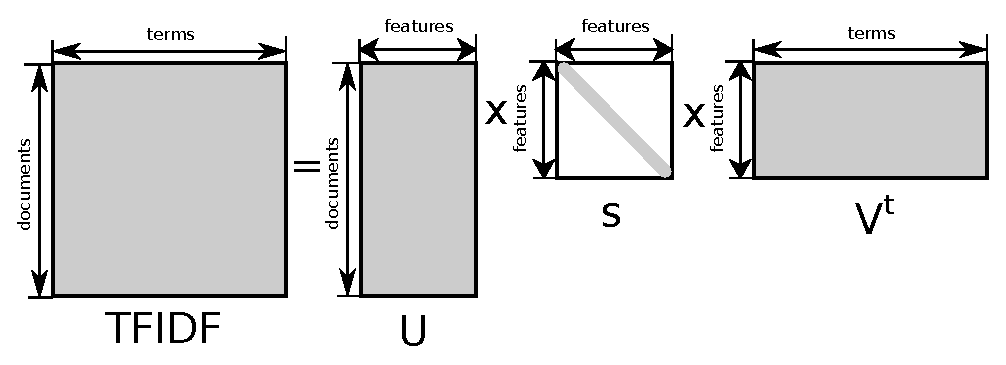
\includegraphics[width=0.9\textwidth]{figures/svd-scheme.eps}
	\caption{Decomposition of TFIDF matrix with singular Value decomposition. Note that $s$ is a diagonal matrix with the singular values sorted in descending order.}
	\label{fig:svd-scheme}
\end{figure}

This way, a reduced feature space is defined, which properly manages noise and redundancy of terms. User profiles are generated from this feature-space definition through a linear combination of document profiles that they liked \cite{Bambini2011}. Then, recommendations are generated comparing user and document profiles with cosine correlation coefficient.

\subsection{Context-aware recommender systems.}

In addition to the information traditionally used by recommender systems, as noted by R.Burke \cite{Burke2002}, other sources of information can be considered in the recommendation, such as the context in which the recommendation is received by users. F. Ricci \cite{Ricci2012contextualizing} stated that the conditions or circumstances in which the recommendation is delivered significantly affect users' decision behavior. Therefore, the consideration of users' context is key to provide interesting recommendations.

With this regard, the various context-aware recommendation approaches can be classified into three classes \cite{Adomavicius2011}:
\begin{itemize}
	\item Pre-filtering: The system selects and uses only the feedback gathered in the same context in which the recommendation is delivered to the user.
	\item Post-filtering: The recommendations are generated first without considering contextual information. After that, the item predictions are modified regarding the specific context of the users, possibly filtering out some items.
	\item Contextual modeling: The contextual information is directly integrated in the model that is used to recommend.
\end{itemize}

In pre-filtering, the approach is to filter out the information that was not not gathered in the current context. In traditional recommender systems the information is viewed as a function $R: User \times Item \rightarrow Rating $ that the recommender system tries to approximate. In CA, the information can be viewed as a three dimensional cube $User \times Item \times Context \rightarrow Rating$. Contextual pre-filtering selects only the information relative to the context, hence, it tries to approximate function $R_{context}: User \times Item \rightarrow Ratings_{context}$ This way, they only consider ratings generated in the context in which the recommendation is delivered to the user. Contextual pre-filtering is a simple and effective approach, but it is affected by data sparsity when there is not enough information generated in all contexts to provide accurate recommendations. Some researchers have tried to overcome this issue through context-generalization \cite{Adomavicius2011} when the information available in the current context is not enough and include information from the broader context.

In post-filtering, the recommendations are first computed overlooking the contextual information, as in traditional recommender systems. After this initial step, recommendations are adjusted to the current context either removing irrelevant items or through a weighting function that updates predictions regarding the suitability of items to target user's context. A previous work \cite{Panniello2009} evaluated them in the same scenarios and compared pre- and post-filtering approaches. It determined that neither pre-filtering nor post-filtering completely dominates the other and a study to determine the best approach is needed in each specific case.

Previous approaches try to reduce the CA problem to a two dimensional one that can be solved with traditional recommender systems. This is not the case in contextual modeling, in which contextual information is directly integrated in the recommendation model to recommend. With this regard, researchers have explored heuristic-based \cite{Panniello2014}, probabilistic \cite{Adomavicius2005b}, or matrix factorization \cite{Baltrunas2011c} contextual modeling approaches.

\subsection{MapReduce and Spark}
\label{sec:background-mapreduce-and-spark}

MapReduce \cite{Dean2008} is a processing tool to manage data in an scalable way. It was originally designed by Google in 2003 aiming to support the most powerful search-engine on the internet, but later it was also applied for parallelization in general purpose applications. In MapReduce (see Figure \ref{fig:background-mapreduce}), two main operations are defined by the user: \emph{Map} and \emph{Reduce}. The \emph{Map} operation takes an input, which is given as a set of $<$key,value$>$ pairs, and produces an intermediate set of $<$key,value$>$ pairs that can be of different type and are defined by the user. An intermediate phase merges all pairs that have the same key and redistributes the work. The \emph{Reduce} operation combines pairs by key to produce a smaller pair set.

\begin{figure}[h]
	\centering
	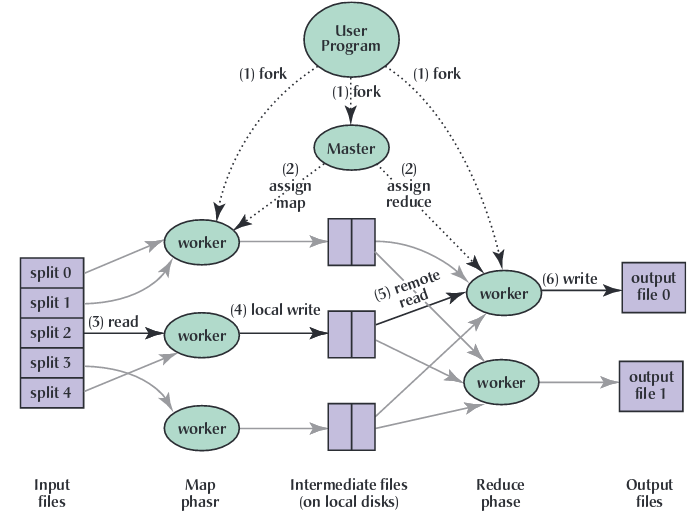
\includegraphics[width=0.95\textwidth]{figures/mapreduce.png}
	\caption{Scheme of the MapReduce approach \cite{Dean2008}.}
	\label{fig:background-mapreduce}
\end{figure}

\revise{Modificar esta figura para hacerla mas adecuada a lo que se explica}

There are several solutions that apply the MapReduce approach. Among them, Apache Spark \cite{Zaharia2016}, which was introduced as part of the Hadoop Ecosystem, offers to the user a set of in-memory primitives that complement the MapReduce ones and that is suitable for iterative tasks. It is based on Resilient Distributed Datasets (RDDs), a structure that stores data in such a way that later computations can be easily parallelized in distributed machines. RDDs allow to cache or redistribute intermediate results, which enables the design of data processing pipelines.

Within Spark we use two libraries: MLlib and Spark streaming. MLlib is a scalable machine learning library \cite{Meng2016} that was built to take advantage of Spark suitability for iterative tasks and provides several machine learning techniques for classification, optimization, and data pre-processing, among others. Specifically, we use the tools that MLlib provides for regression and clustering. Spark Streaming \cite{Chintapalli2016} provides an scalable way to manage data produced at high rates, which allow us to handle the data provided by microblogging systems and compute the context model.

\section{Semantic model for recommending questions with context awareness based on topic detection in collaborative interest}
\label{sec:proposal}

Here, a novel proposal, LSAContextCluster, for recommendation based on CA-CB is introduced. Recommendations might need to be targeted to specific contexts, e.g., when a system delivers recommendations of answers in the history domain and currently people are posting about Colombus Day, then the system should promote answers related to the discovery of the Americas. In this kind of cases, it is possible to modify user profiles to include contextual information in such a way that later recommendations are both targeted to user preferences and current context.

The proposed model fits into the CA approach of contextual modeling, because it integrates contextual information in the model built by the recommender system. The general scheme of the proposal, LSAContextCluster, is depicted in Figure \ref{fig:proposal-scheme}, and it is composed of five phases:
\begin{enumerate}[(i)]
	\item QA domain semantic analysis: It applies LSA to reduce the dimensionality of the term-document matrix.
	\item Build user's preference profile: It analyses users' preferences and generates a profile for each of them based on the profiles of the document he/she liked in the past.
	\item Build context model: It analyses the context, which consists on a stream of status updates within a given time frame, applies clustering to separate the various topics that the context contains, and generates feature-space profiles for each context topic.
	\item Contextualize user profiles: It selects the context topic that is most suitable to target user's preferences and combines the preference-based user profile with the context topic profile to generate the contextualized user profile.
	\item Prediction: It compares the document profiles and the contextualized user profile to recommend.
\end{enumerate}

\begin{figure}[h]
	\centering
	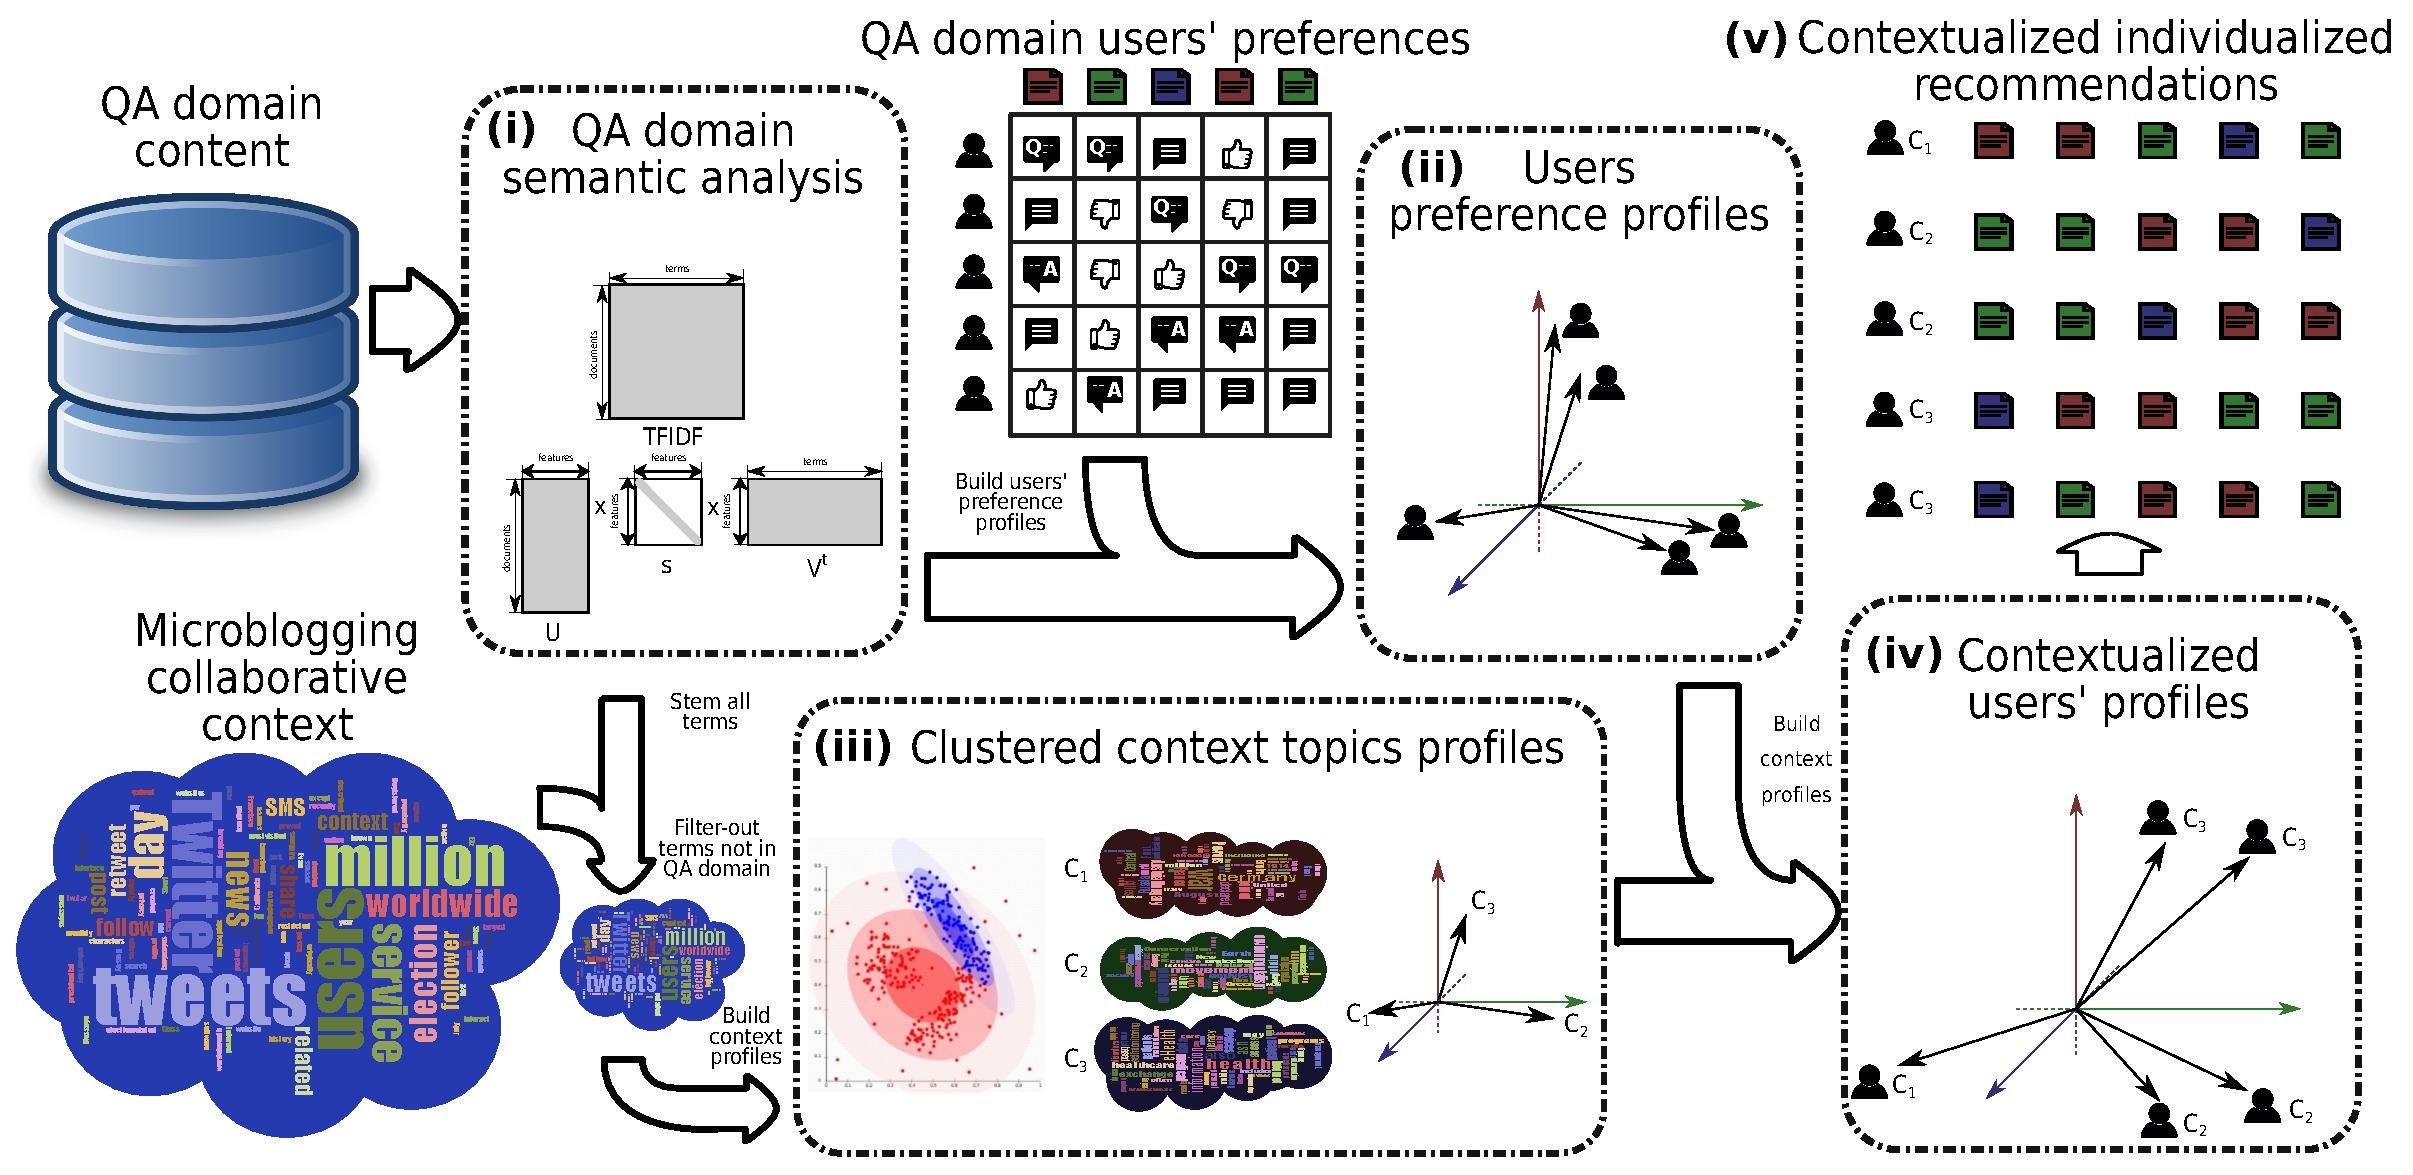
\includegraphics[width=0.95\textwidth]{figures/proposal-scheme-v5.eps}
	\caption{General scheme of the proposal.}
	\label{fig:proposal-scheme}
\end{figure}

\subsection{QA domain semantic analysis}
\label{sec:proposal-qa-semantic-analysis}

Our proposal assumes that the QA dataset contains textual information of the question and their related answers. In this proposal we consider the questions together with all their answers as the document, and the words used in their text as the terms. The terms are stemmed using the Porter Stemmer algorithm \citep{Porter1980}. Once terms are stemmed, the TFIDF document profiles $profile^{TFIDF}_{d}$ are built according to Eq. \ref{eq:document-profile-tfidf}.

Once the TFIDF document profiles are built, LSA is performed to reduce the dimensionality of the matrix. LSA is proven to be effective through the description of both document and terms in a feature space with a reduced number of features. Therefore, the aim of this step is to decompose the initial word-document matrix in a word-features matrix $U$, a singular value vector $s$, and a document-features matrix $V$ (see Eq. \ref{eq:svd}).

An approximated factorization of the TFIDF matrix is performed with Singular Value Decomposition, which allows to reduce the dimensionality of the original matrix keeping the $f$ most relevant singular values of the original matrix. Hence, we obtain the profile of both terms and documents in the feature space, which compose the QA domain semantic model:

\begin{equation}
	profile^{LSA}_d = \{ u_{t,1},\dots, u_{t,f}\}
\end{equation}
\begin{equation}
	profile^{LSA}_t = \{ v_{t,1},\dots, v_{t,f}\}
\end{equation}

\subsection{Building user preference profile}

At this point LSAContextCluster has built a model with terms and documents profiles. In order to provide personalized recommendations to users, it is needed to build user profiles in the same feature-space. LSAContextCluster holds a unary matrix that states whether a given user has expressed interest in another document (see Table \ref{tab:user-preferences}) either creating, commenting, or voting it. In this table, the set of documents that user $u$ has expressed interest in is defined as:
\begin{equation}
	R_{u} = \{d ~~~~s.t.~~~~r_{u,d} \in R \}
\end{equation}

\begin{table}
	\caption{Users' preferences over items, the rating matrix.}
	\label{tab:user-preferences}
	\centerline{\small\baselineskip=13pt
	\begin{tabular}{|c||ccccc|}
		\hline
         &     $d_1$     & $\dots$  &     $d_k$     & $\dots$  & $d_n$
		\tabularnewline
		\hline
		\hline
$u_1$    & $r_{u_1,d_1}$ & $\dots$  & $r_{u_1,d_k}$ & $\dots$  & $r_{u_1,d_n}$
		\tabularnewline
$\vdots$ & $\vdots$      & $\ddots$ & $\vdots$      & $\ddots$ & $\vdots$
		\tabularnewline
$u_j$    & $r_{u_j,d_1}$ & $\dots$  & $r_{u_j,d_k}$ & $\dots$  & $r_{u_j,d_n}$
		\tabularnewline
$\vdots$ & $\vdots$      & $\ddots$ & $\vdots$      & $\ddots$ & $\vdots$
		\tabularnewline
$u_m$    & $r_{u_m,d_1}$ & $\dots$  & $r_{u_m,d_k}$ & $\dots$  & $r_{u_m,d_n}$
		\tabularnewline
		\hline
	\end{tabular}}
\end{table}

This way, the user's profile is built upon the profiles of the documents that belong to $R_u$, and describes the user's preferences in terms of the latent space:
\begin{equation}
	profile^{LSA}_u = \sum_{d \in R_u} profile^{LSA}_d = \{ \sum_{d \in R_u} profile^{LSA}_{d,1}, \dots, \sum_{d \in R_u} profile^{LSA}_{d,f}\}
\end{equation}

The user's profile does not need to be normalised because it is later compared with other profiles using cosine correlation coefficient, which only considers the angle of the vectors being compared.

\subsection{Context model building}

To include contextual information in the recommendation process, it is needed to build the context model. In this proposal, we aim to promote questions that are relevant regarding current happenings. With this regard, our proposal uses status updates from microblogging services, such as Twitter, as the source of collaborative interest. Formally, a status update consists of a free text input generated by a user with certain timestamp, among other meta-data. Analyzing these status updates, LSAContextCluster generates a model of the context that is later used to modify the user profile. The scheme of the context model building phase is depicted in Fig. \ref{fig:proposal-context-clustering-phase}.

\begin{figure}[h]
	\centering
	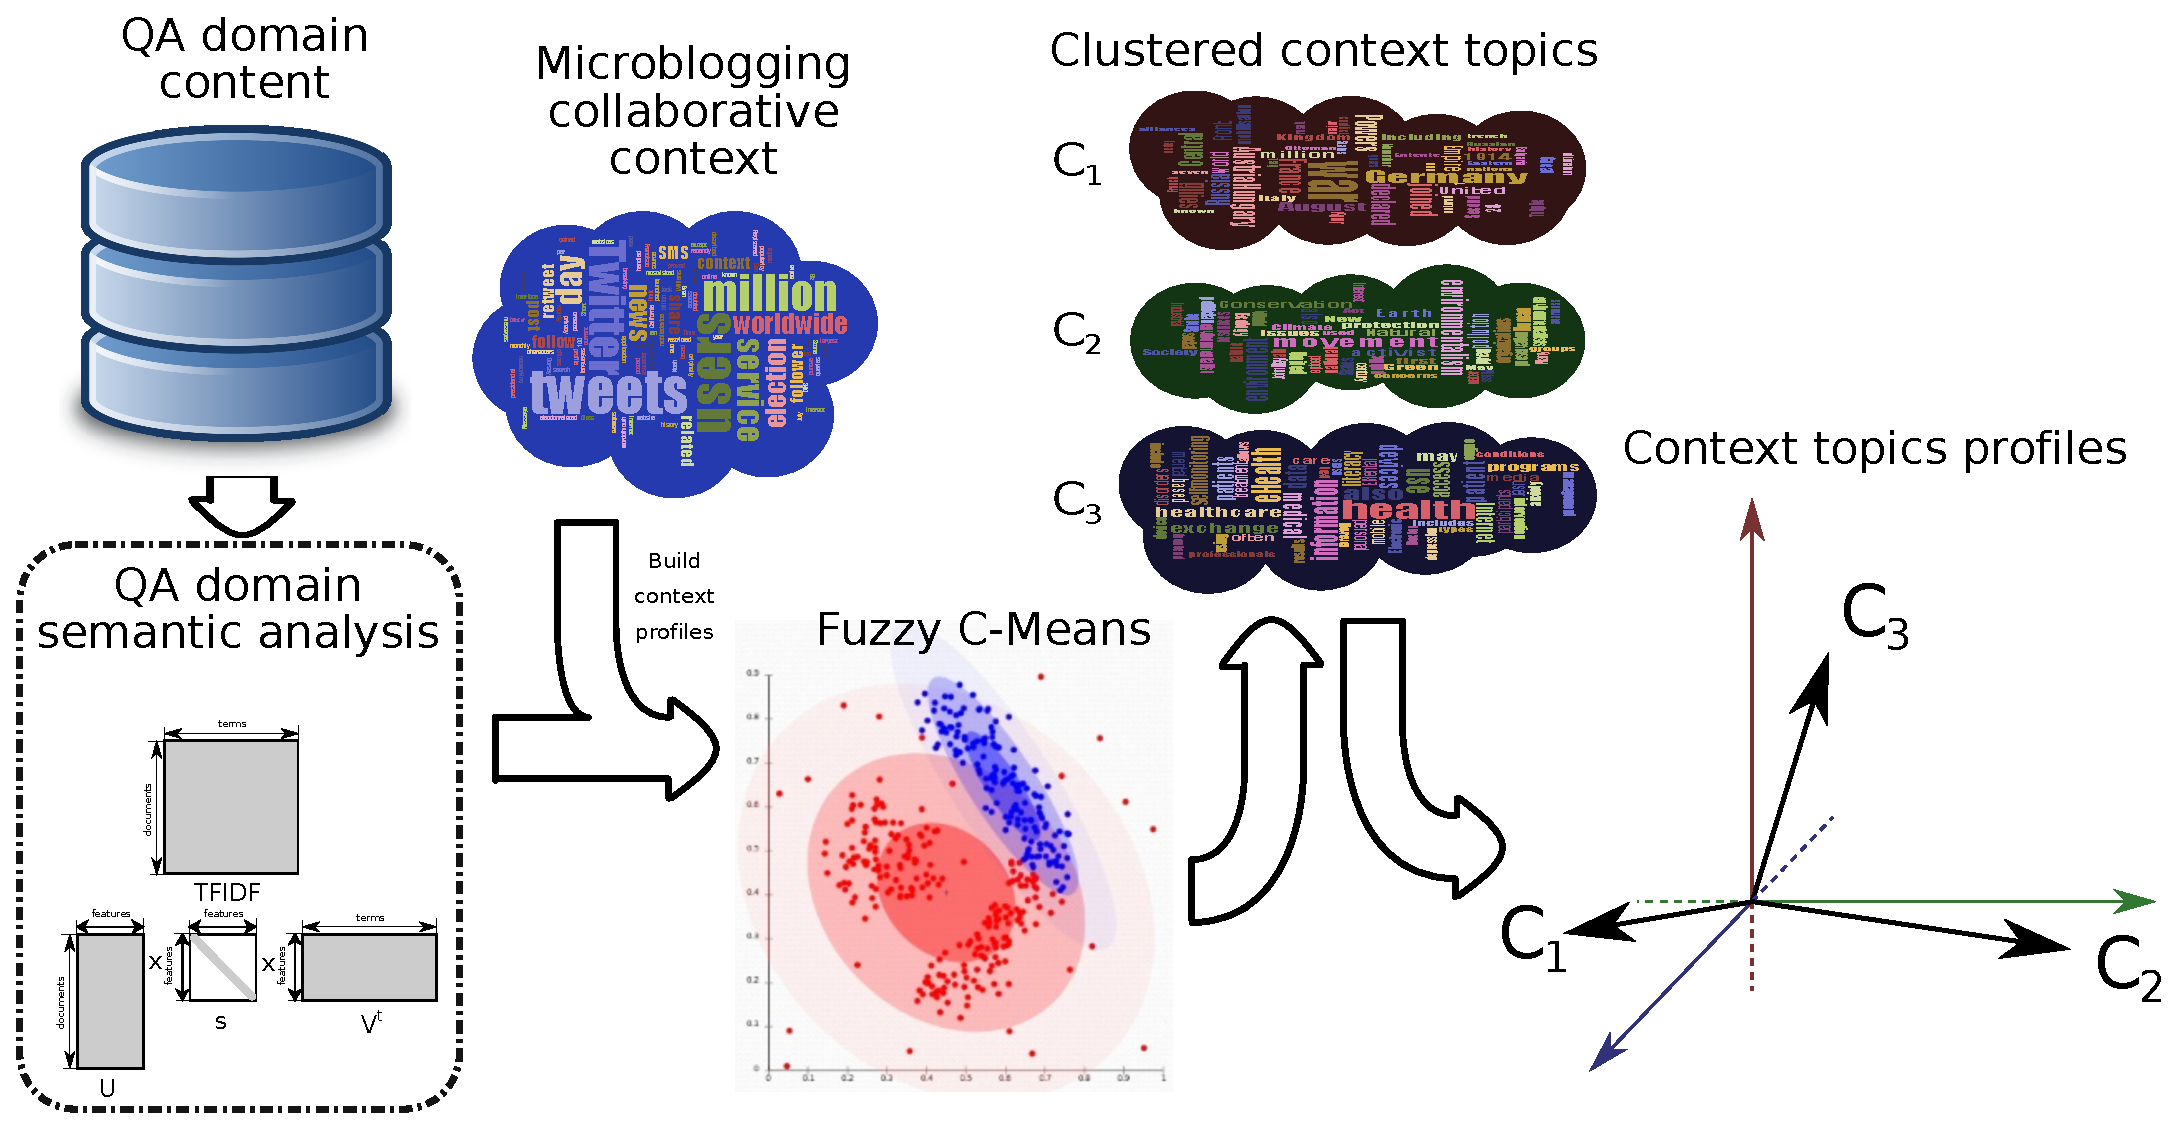
\includegraphics[width=0.95\textwidth]{figures/clustering-phase.eps}
	\caption{Context model building phase.}
	\label{fig:proposal-context-clustering-phase}
\end{figure}

The context is composed of the status updates that were generated in a given time window, which is set to 24 hours in this proposal, although it could be modified to adjust the sensitivity of the context model. First, all terms of the status updates of the current context are stemmed. After that, from all the terms that the context contains, LSAContextCluster filters out the terms that do not appear in the QA semantic model generated in phase one (see Section \ref{sec:proposal-qa-semantic-analysis}).

Given that the context is composed of several status updates, there can be a mixture of topics. To determine the context topics, the proposal performs a fuzzy clustering of the terms used in the context. Hence, fuzzy c-means clustering algorithm \cite{Bezdek1984} groups the terms using their feature vector $profile^{LSA}_t$ as the term definition. The distance among terms used in the clustering is based on cosine correlation coefficient. The result is a set of clusters where each cluster  $c_i$ defines a context topic.

Once the terms of current context are grouped in context topics, the proposal generates a context profile for each topic combining the profiles of the terms that are included in each cluster. Therefore, LSAContextCluster builds a profile for each context topic using the feature representation of each term from the QA domain (see Eq \ref{eq:context-topic-profile}). At the end of this phase, LSAContextCluster has generated a model of the context composed of several context profiles, one for each context topic detected by the clustering.

\begin{equation}
	profile^{LSA}_{c_i} = \sum_{t \in c_i} profile^{LSA}_{t}=\{\sum_{t \in c_i} profile^{LSA}_{t,1}, \dots, \sum_{t \in c_i} profile^{LSA}_{t,f} \}
	\label{eq:context-topic-profile}
\end{equation}

\subsection{User profile contextualization}

In this step, the target user's preference profile is combined with the context model to provide contextualized personalized recommendations. To do so in a personalized way, from all the context topic profiles that the context model contains, LSAContextCluster selects the most similar to the user's preference profile. This way, the context topic $c_i$ that has a greater cosine coefficient with the target user preferences is used to modify his/her profile, hence, the contextualization of user profiles is personalized to user preferences.

\begin{equation}
	\argmax_{c_i}~~~~ cosine(profile^{LSA}_u,profile^{LSA}_{c_i})
\end{equation}

After this selection, the profile of the selected context topic $c_i$ and the user's preference profile are combined to obtain the contextualized user profile. With this regard, the convex combination is applied, which allows to perform a weighted combination regulated by $\alpha$ parameter -- the greater its value, the more importance of the user's preference profile over the profile of the selected context topic in the contextualized user profile.

\begin{equation}
	profile^{LSA}_{C,u} = \alpha * profile^{LSA}_u + (1- \alpha )*profile^{LSA}_{c_i}
\end{equation}

\subsection{Prediction}

Once we have the contextualized user profile, we can produce a prediction of the suitability for a given item regarding the profile. The recommendation is a list of documents sorted by $p_{u,d}$:

\begin{equation}
	p_{u,d,c} = profile^{LSA}_{C,u}*s*profile^{LSA}_d
\end{equation}

\section{Case study and experiment}
\label{sec:case-study}

To evaluate the proposal, we performed an experiment that simulates the recommendation of QA items in various contexts. The remainder of the section is structured as follows. First, the settings of the experiment are described. The datasets and methods for processing them are then detailed. After that, the evaluation measures are commented. Lastly, the results are analyzed.

\subsection{Experimental procedure}

In these experiments we compared several CB approaches based on LSA with contextual information. In order to do the experiment, the procedure proposed by Sarwar et al. \cite{Sarwar2001}  was performed with modifications to consider contextual information in the experiment:
\begin{itemize}
	\item Split the dataset in training and test.
	\item Build the model with training data.
	\item Build the profile of each user including contextual information if applicable.
	\item Recommend to each user based on their profile and the model.
	\item Evaluate recommendations with the test set.
\end{itemize}

This procedure was repeated 20 times and 5-cross fold validation was used to split the data in training and test sets. Moreover, various contexts were considered, which are detailed in Section \ref{sec:case-study-datasets}.

\subsection{Methods compared}

The baseline method to compare with was the LSA method without contextual information. For the sake of fair comparison, the number of features was fixed in all models, and 30 features were considered in LSA.

We compared several ways for integrating contextual information in QA recommendation. Here, we show the results of three ways to characterize the context:

\begin{itemize}

	\item No clustering (LSAContext): The words are not separated in clusters, therefore the context profile is unique. There is a single profile of the context that is built combining the profiles of the words that are included in the context.
	\begin{equation}
		profile_{C} = \sum_{t \in C} * profile_t
	\end{equation}

	\item Weighted by membership (LSAContextClusterFuzzy): The cluster profiles are built combining the feature vector of each word weighted by the membership value of the word to the cluster:
	\begin{equation}
		profile_{c_i} = \sum_{t \in c_i} \mu_{t,c_i} * profile_t
	\end{equation}
	\noindent where $\mu_{t,c_i}$ is the membership of term $t$ to cluster $c_i$.

	\item Max membership (LSAContextClusterMax): The words are used only in the cluster to whom they have the highest membership value:
	\begin{equation}
		profile_{c_i} = \sum_{t \in T} \mu^{max}_{t,c_i} * profile_t
	\end{equation}
	\noindent where $\mu^{max}_{t,c_i}$ is one if $\mu_{t,c_i}$ is the maximum membership across clusters, and zero otherwise.

\end{itemize}

Moreover, in order to adjust the weight of preference profile over context profile, the methods compared have parameter $\alpha$. In the experiment we explored several values for it, here, to make the results clearer, we show only $\alpha \in [0.90,1.00]$ with increments of $0.01$.

\subsection{Datasets}
\label{sec:case-study-datasets}

In the experiment there are two sources of data: The QA domain and the contextual information.

The QA domain used is the StackExchange dataset\footnote{http://data.stackexchange.com/}. This dataset consists of the database dump of each site in the stackexchange ecosystem. Across them, we focus on 3dprinting, a StackExchange site devoted to it. Some stats are detailed in Table \ref{tab:stackexchange-dataset-description}.

\revise{Luis: Un monton de marcas que no entiendo... (i) it would be nice to clarify ........... dataset, (ii) sobre algo de at this stage}

\begin{table}
	\caption{Main features of the QA domain datasets used in the case study.}
	\label{tab:stackexchange-dataset-description}
	\centerline{\small\baselineskip=13pt
	\begin{tabular}{l|rrrrrr}
\hline
          & 3dprinting & academia & ai      & android & apple   & history \\
\hline
Users     & 4025       & 48448    & 3158    & 119810  & 145011  & 13433   \\
Questions & 597        & 57967    & 421     & 41423   & 77978   & 6127    \\
Answers   & 1135       & 16737    & 749     & 49985   & 115643  & 12212   \\
Comments  & 2754       & 40319    & 1165    & 123291  & 242238  & 53510   \\
Votes     & 7860       & 138416   & 5323    & 359710  & 669305  & 162809  \\
Ratings   & 2458       & 119082   & 1461    & 109644  & 241838  & 38082   \\
Sparsity  & 0.99898    & 0.99996  & 0.99890 & 0.99998 & 0.99998 & 0.99954 \\
\hline
	\end{tabular}}
\end{table}

In this experimental setup, the results are reported per StackExchange site. Therefore, we consider each site as a different dataset. Given that the aim of the system is to provide users with pieces of information that help explain the context and also consider their preferences.

Regarding the contextual dataset, a set of interesting keywords is defined based on the aim of the proposal for contextualizing recommendations. Given that the proposal focuses on selecting currently hot topics, we have selected the terms \emph{news}, \emph{current} and \emph{situation}. From these seed terms, we extracted a dataset of tweets that contain any of these words from Twitter. The stats of the dataset extracted is depicted in Figure \ref{fig:context-dataset-description}.

\begin{figure}[htb]
    \centering
    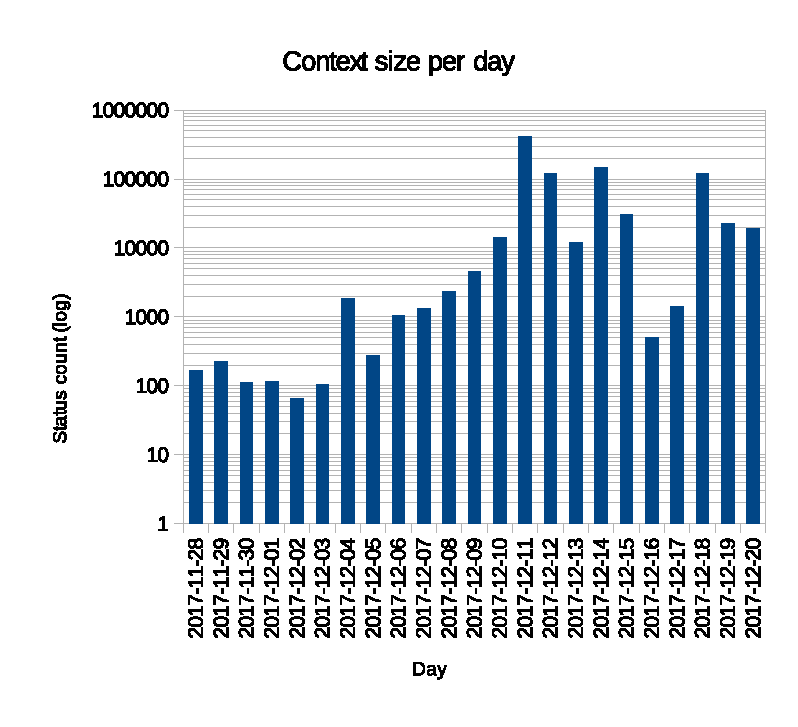
\includegraphics[width=0.9\textwidth]{figures/context-dataset-description.eps}
    \caption{Contextual dataset used in the experiment, where each day has a different status count.}
    \label{fig:context-dataset-description}
\end{figure}

\subsection{Evaluation Measures}

Usually, measures to evaluate the prediction errors in terms of rating deviation are used. However, the methods being compared do not provide a rating prediction, but a value that expresses the suitability of items regarding the user profile. Therefore, the measures that can be used are information retrieval ones, such as precision and recall. Researchers have remarked that, although they are useful, they are not sensible to the sorting of the items that the recommender systems does \cite{Gunawardana2015}. In order to consider the quality of the sorting, the NDCG is used:

\begin{equation}
	DCG_u = \sum_{k=1}^N\frac{r_{u,recom_{u,k}}}{log_2 (k+1)}
\end{equation}

\noindent where $recom_{u,k} \in I$ is the item recommended to user $u$ in $k$ position.

\begin{equation}
	NDCG = \frac{DCG}{DCG_{perfect}}
\end{equation}

\noindent where $DCG_{perfect}$ is a perfect sorting of the items, i.e., the list of items sorted by their value in the test set.

\subsection{Results}

In this section, the results obtained for the different approaches compared are shown and analyzed to evaluate the performance of the proposal. Figures \ref{fig:ndcg-results-proposal-context-no-clustering}, \ref{fig:ndcg-results-proposal-context-fuzzy-clustering-membership}, and \ref{fig:ndcg-results-proposal-context-fuzzy-clustering-max} show the results of the 3 techniques compared in the 3dprinting QA dataset. The three figures have the same scale and, in X axis, alpha parameter is shown. Note that for $\alpha=1.00$ the result correspond to LSA approach because the context profile is ignored. The series denote the context, hence its position shows the results of the proposal with the corresponding $alpha$ value for the day.

\begin{figure}[htb]
    \centering
    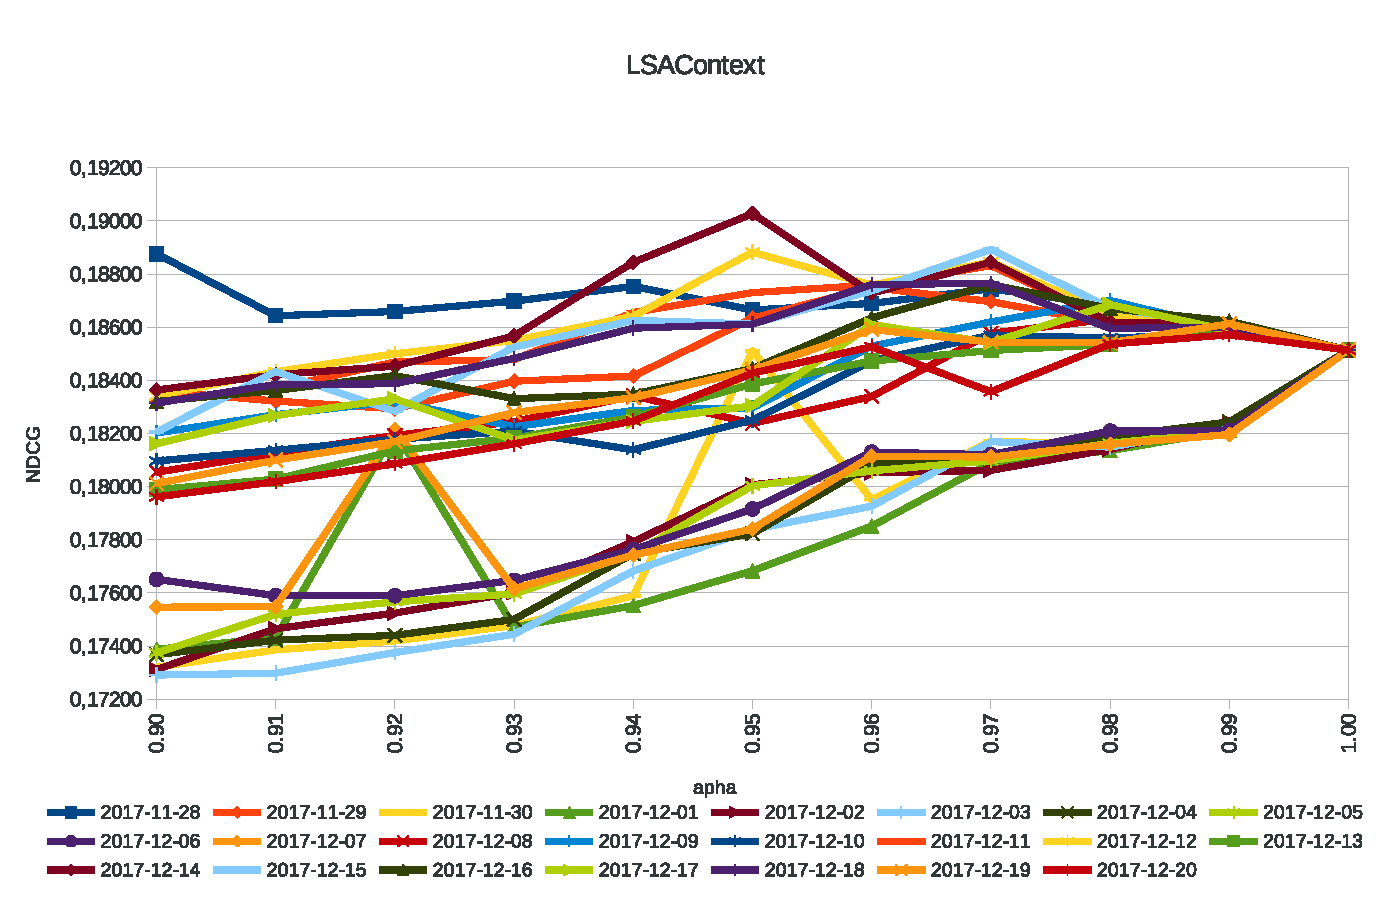
\includegraphics[width=0.98\textwidth]{figures/ndcg-results-proposal-context-no-clustering.eps}
    \caption{Results of the proposal to manage context without clustering}
    \label{fig:ndcg-results-proposal-context-no-clustering}
\end{figure}
\begin{figure}[htb]
    \centering
    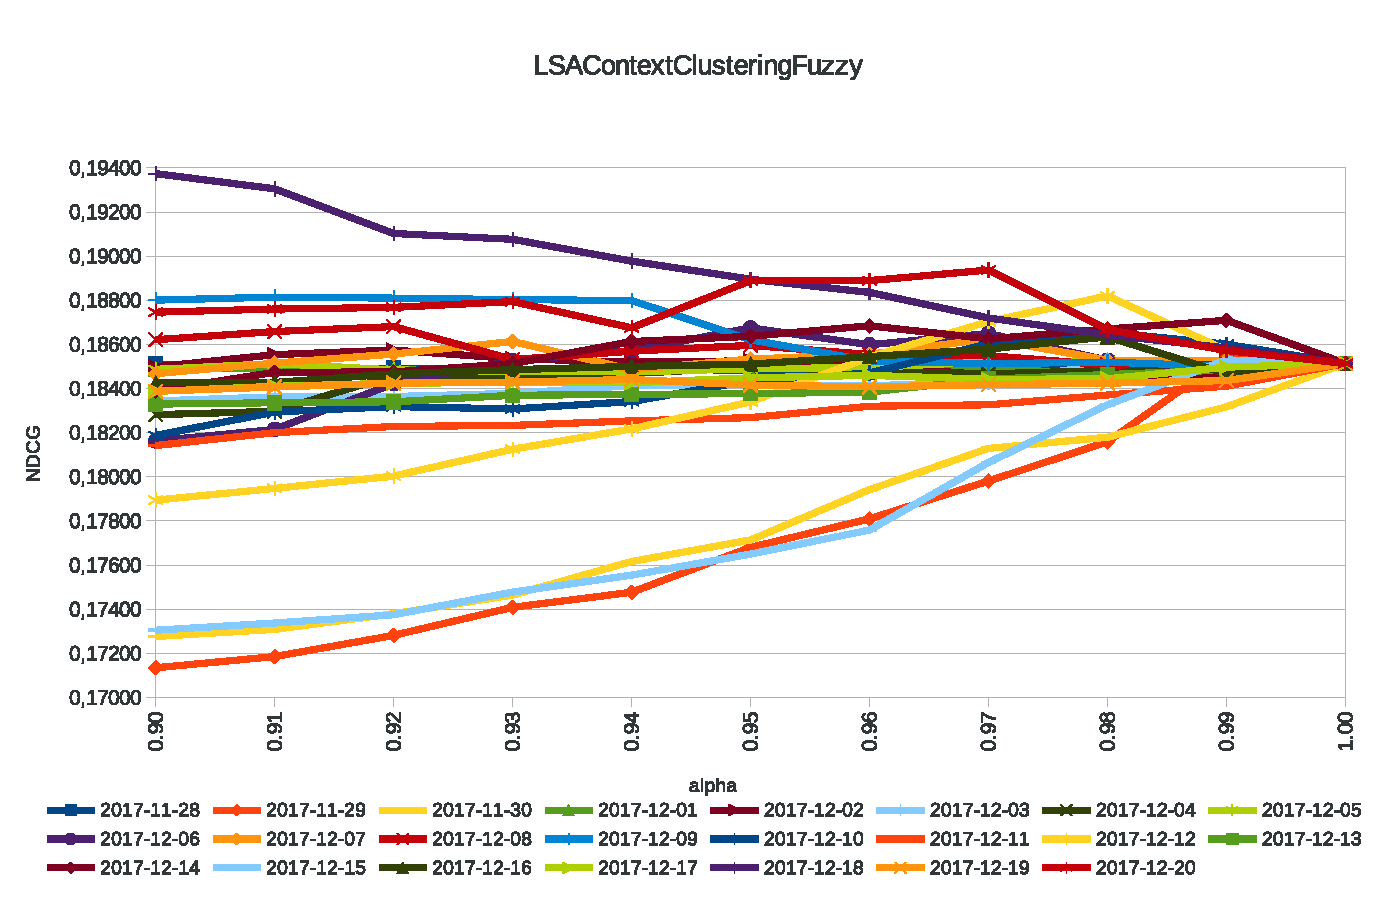
\includegraphics[width=0.98\textwidth]{figures/ndcg-results-proposal-context-fuzzy-clustering-membership.eps}
    \caption{Results of the proposal to manage context with fuzzy membership.}
    \label{fig:ndcg-results-proposal-context-fuzzy-clustering-membership}
\end{figure}
\begin{figure}[htb]
    \centering
    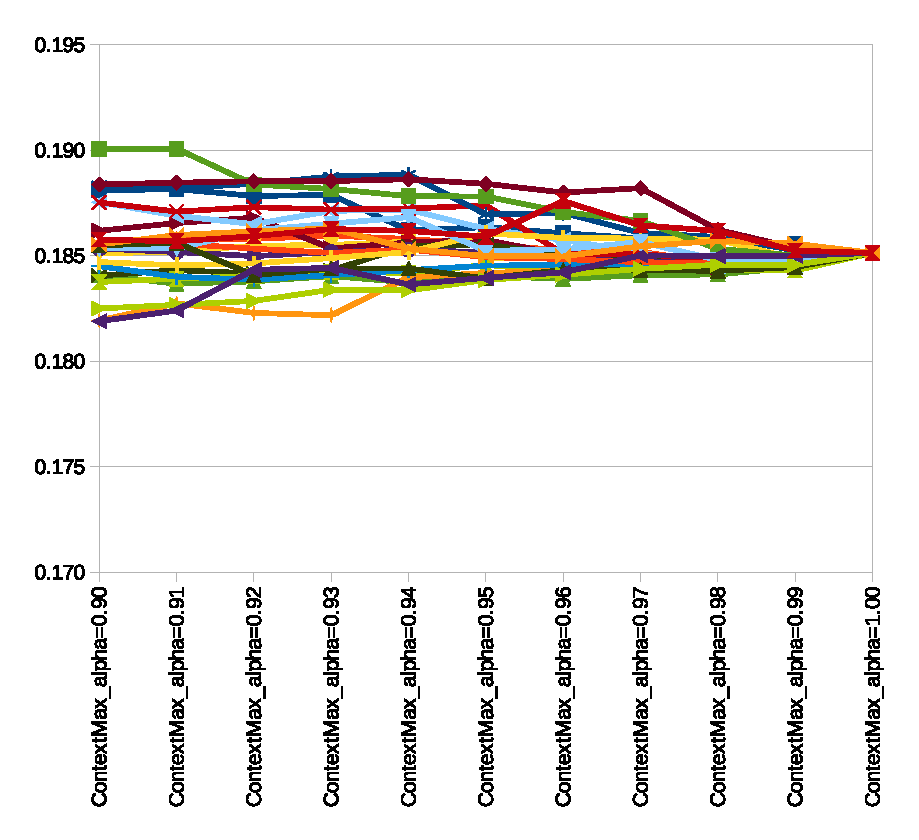
\includegraphics[width=0.98\textwidth]{figures/ndcg-results-proposal-context-fuzzy-clustering-max.eps}
    \caption{Results of the proposal to manage context with max membership.}
    \label{fig:ndcg-results-proposal-context-fuzzy-clustering-max}
\end{figure}

In Figure \ref{fig:ndcg-results-proposal-context-no-clustering} it can be noticed that, although the proposal improves the results of LSA ($\alpha = 1.00$) in some days (contexts), the improvement does not compensates for the decay in performance in other days. Focusing in the context of 2017-11-28, LSAContext improves the results of LSA for all alpha values.

Figure \ref{fig:ndcg-results-proposal-context-fuzzy-clustering-membership} shows that LSAContextFuzzy improves the results of LSA ($\alpha = 1.00$). It obtains better results than LSAContext, given that the results are distributed higher than those of the LSAContext approach. If we focus on the results on single days, it can be noticed that LSAContextFuzzy improves greatly for the context of day 2017-11-28. However, there is a major decay in three contexts: 2017-11-29, 2017-11-30 and 2017-12-15 in which the proposal does not even reach the value of the LSA approach. If we focus specifically on the day 2017-12-12, there is a decay for $\alpha \in [0.90,0.95]$ but it improves the results of LSA for $\alpha \in [0.96,0.99]$.

Figure \ref{fig:ndcg-results-proposal-context-fuzzy-clustering-max} shows that LSAContextClustering improves the results of LSA ($\alpha = 1.00$) for most of the contexts explored. It consistently obtains better results than LSA, although the improvements obtained in some contexts is canceled with worst results in other contexts.


Figure \ref{fig:ndcg-results-3proposals-bests-per-day} compares the results of each proposal with the best alpha. Here LSA has no variability across days because it does not considers context. LSAContext has a great variability in performance across days, however, the better results obtained from 2017-12-08 onwards are canceled by the low performance from 2017-11-30 to 2017-12-07. LSAContextClusteringMax and LSAContextClusteringFuzzy performances did not dropped drastically in certain contexts as it happened for LSAContext. Instead, they show ups and downs in the contexts. It is worth to notice that LSAContextClusteringMax obtained greater peaks than LSAContextClusteringFuzzy.

\begin{figure}[htb]
    \centering
    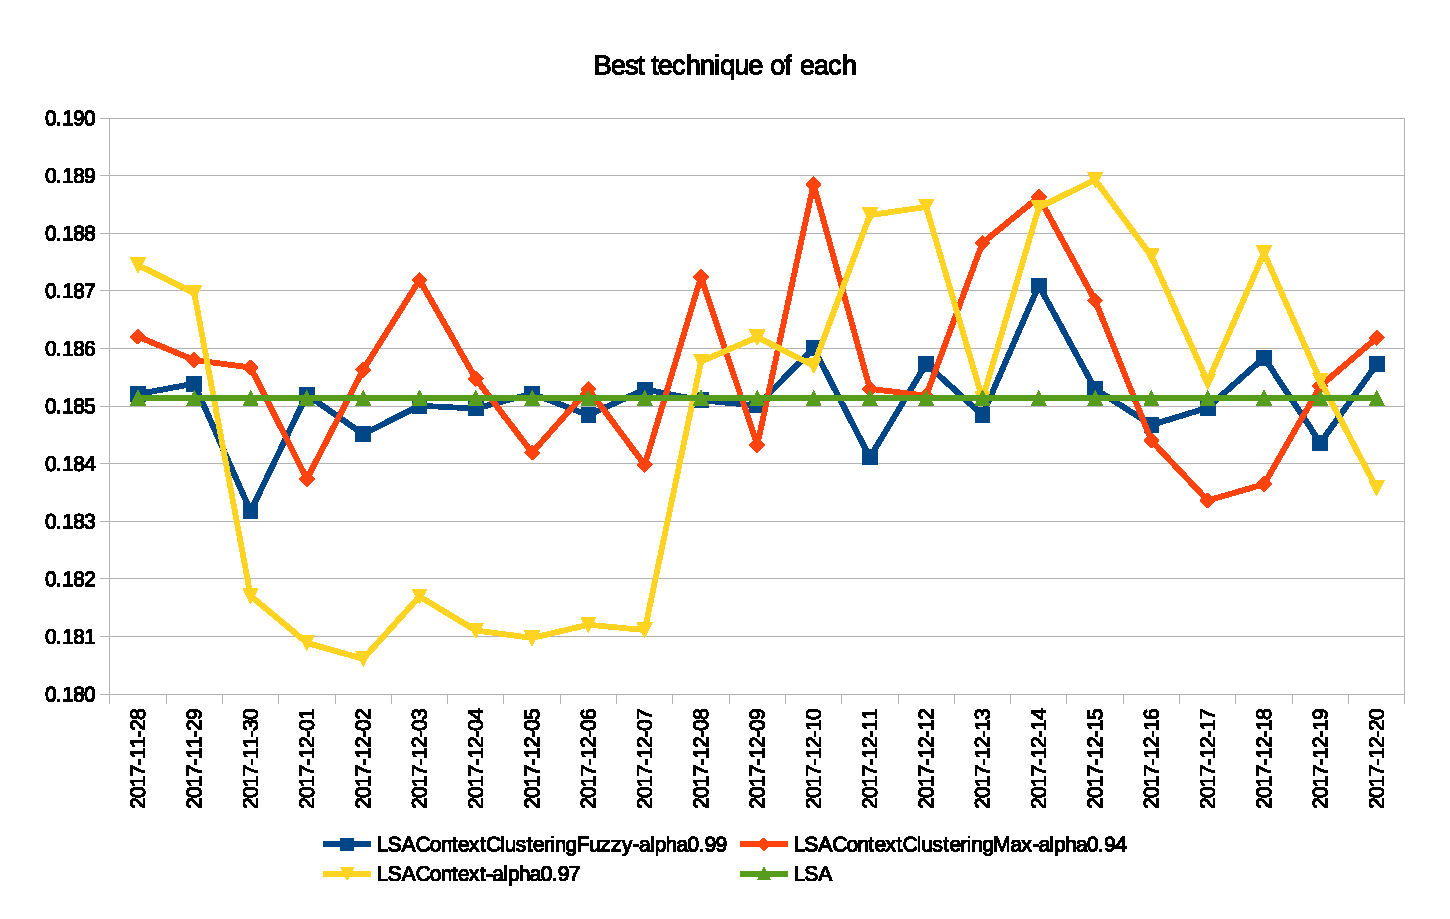
\includegraphics[width=0.98\textwidth]{figures/ndcg-results-3proposals-bests-per-day.eps}
    \caption{Results of the proposal to manage context with fuzzy membership.}
    \label{fig:ndcg-results-3proposals-bests-per-day}
\end{figure}

Figure \ref{fig:ndcg-results-3proposals-average} summarizes the results of the three proposals as compared to the LSA approach. It shows that LSAContextFuzzy and LSAContext, although they obtain better results than LSA in some contexts, in average they do not provide improvement. In the case of LSAContextClustering, it overcomes the results of all the remaining approaches for $\alpha \in [0.90,0.97]$. For $\alpha=0.94$ it reached the maximum average NDCG across all contexts explored, hence this value is the best one in this QA domain.

\begin{figure}[htb]
    \centering
    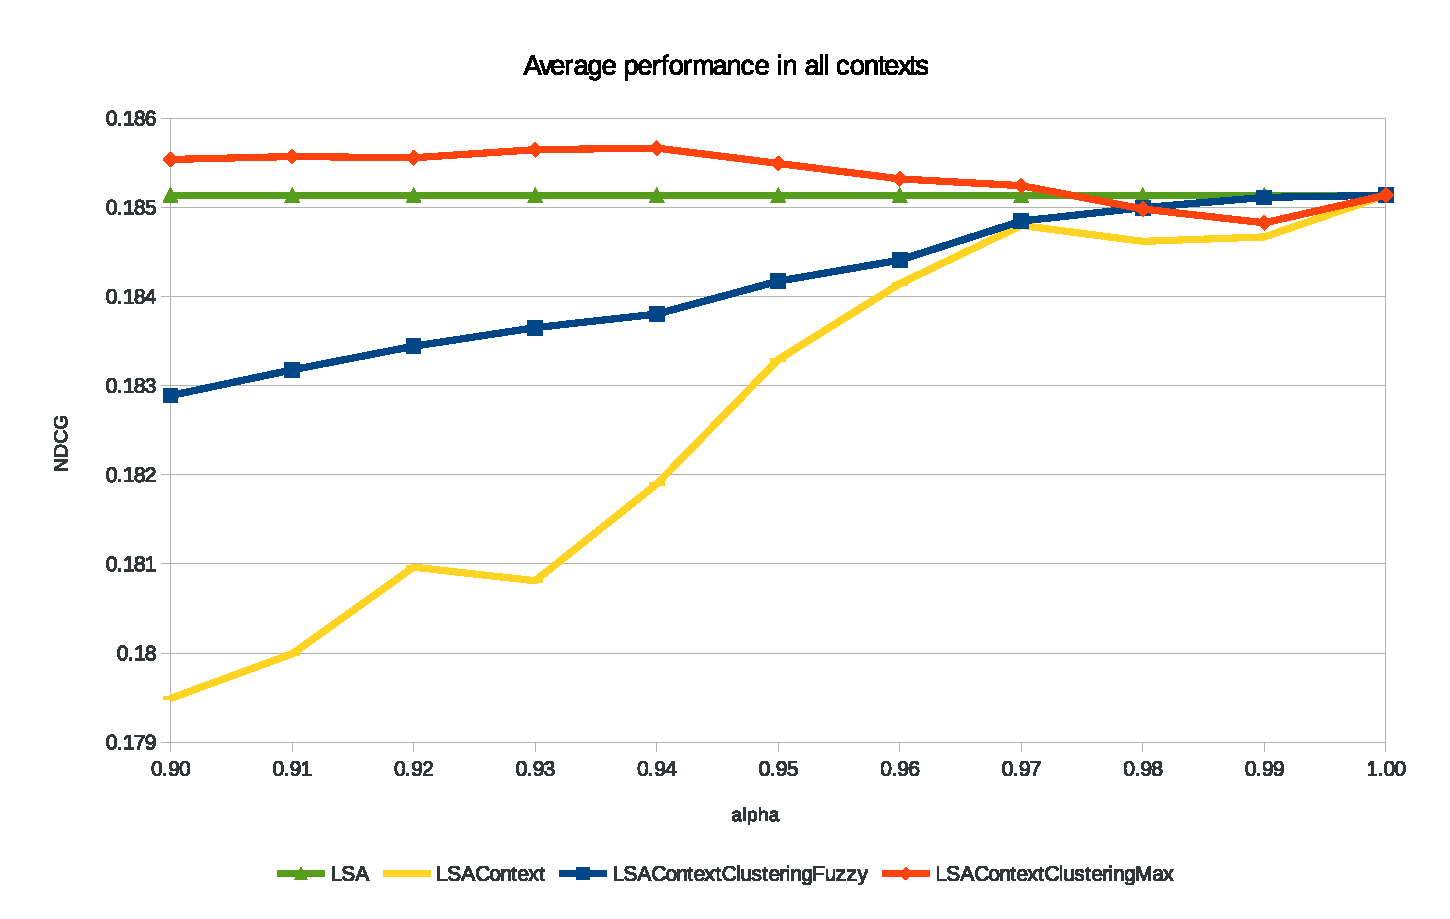
\includegraphics[width=0.9\textwidth]{figures/ndcg-results-3proposals-average.eps}
    \caption{Average NDCG of the compared approaches in all contexts.}
    \label{fig:ndcg-results-3proposals-average}
\end{figure}

The best approaches of the compared ones is the LSAContextClustering with $\alpha=0.94$. This value has been optimized for the 3dprinting QA dataset, hence, for other domains it needs to be adjusted. This parameter provides the LSAContextClustering with flexibility to adapt to different QA domains.

\section{Conclusions and further study}
\label{sec:conclusions}

In this paper, we have explored the application of contextual information in the QA domain recommendation. LSAContextClustering first builds the LSA model associated to the QA domain. After that, it builds the user profile combining the QA profiles with the user preferences. In parallel, it builds the profiles of the context, which is separated in a number of clusters and a context profile is built for each of them. The following step is to combine the user profile with the context profile that is more close to their preferences, which is achieved computing the cosine coefficient between the profiles. This combined profile allows the system to know user preferences and also consider contextual information in the recommendation. 

We performed a case study to compare various configurations for the proposed approach. It shows that all improvements done provide better results as compared to the baseline method (LSA). We found out that the best way to generate each context cluster profile is to select only the words whose membership value is the highest across clusters in the explored QA domain.

In this scenario, contextual information is a key source of information to provide users with relevant recommendations that allow them to better understand the current scenario. The provided system is a relevant tool in the completion of user knowledge through the recommendation of QA items.

\textbf{\textit{Acknowledgements:}} This research work was partially supported by the Research Project TIN-2015-66524-P, the Spanish FPU fellowship (FPU13/01151).

\section*{Bibliography}
\bibliography{rs-bibliography}
\bibliographystyle{plain}

\end{spacing}

\end{document}